\chapter{Software development and management processes}
The following chapter explains the software development and management processes that were employed throughout the project. In the following section some of the necessary terminology will be introduced and explained. Subsequently the process description will be given, followed by a comparison to established process models.

\section{Terms}
Here follows a description of terms as used in the current project.

\begin{description}

\item[Agile methods] \label{def:agile} are a set of software development methods that emphasize on adapting to change over following a predetermined plan, continuous customer collaboration over contract negotiation and implementation over documentation.

\item[Extreme programming] (XP) is an agile software development methodology which favors improving the code and quick responses to customer desires. The customer is involved with the process continuously, and keeps giving feedback on the most recent progress. Releases of new code is also supposed to happen often, so both the customer and the developers are aware what the current progress is, and can give feedback on it. Both the code and requirements are expected to change during the development process. It is incremental in that what the customer wants is implemented swiftly, and stays as a part of the code. It is iterative in that code that is added will likely be subject to change and refactoring during the development process. Constant refactoring and pair-programming is made use of so the quality of the code will be kept as high as possible, as code-quality it will be difficult to plan and design for code-quality. 
% like Iterative development except it is faster. Extreme programming uses a cycle based programming system like the Iterative approach. Unlike the Iterative approach it has a checkpoint after each stage, where the code is being released and new customer requirements is added. The customer are often intimately involved in prioritizing and specifying the requirements. Extreme programming enables the possibility to make it so that several developers can produce code, integrate and test it on the same day.  %TODO: FIX
Iterative development] \label{def:incrementalDev} is an approach to software development that is "based on the idea of developing an initial implementation, exposing this to user comment and evolving it through several versions until an adequate system has been developed"\footnote{Sommerville, p32 \cite{sommerville}}. Benefits to iterative development include adaptability to changing requirement and facilitation of feedback. In the negative side, it can be hard to keep an overview of the progress of the entire system, making it harder to plan ahead for deadlines.

\item[Pair programming] \label{def:pairprogram} is a programming technique taken from XP. In PP, coders work in pairs that work on the same workstation. As each line of code is looked at by at least two people, code development simultaneously acts as a review process, making code developed by a programmer pair more reliable and readable than code developed by an individual programmer. For complex coding tasks, the productivity of a programmer pair is normally higher than that of two individual programmers, considering the reduced effort required for bug fixing. For routine tasks, however, productivity is lower in a programming pair.

\item[Plan-driven development] \label{def:plan-driven} is an approach to software development that recommends careful planning of the software development process, work breakdown and scheduling before starting the implementation process. 

\item[Sprint] \label{def:sprint} is the period unit in which work is planned and done. It is customary to operate with sprints of 2-4 weeks, but the current project operated with sprints of 1-2 weeks.

\item[Spike] \label{def:spike} is a sprint spent primarily or solely on non-programming activities, such as research, documentation or planning.

\item[Stand-up] \label{def:dailyScrum} is a meeting in which all the group members explain shortly what they have been doing since the last meeting, what they are planning to do until next time, and any help or advice they need to continue. Stand-ups function as a binding factor that keeps the entire group on the same page, and provides flexibility by giving the opportunity to change the plans and tasks partway through the sprint.

\end{description}

\section{Development process}
\label{def:devProcess}
The customer required an incremental development process where ideally a new version of the product could be demonstrated at every weekly customer meeting. Furthermore, plans for the following week were to be sketched in collaboration with the customer at the weekly meeting. With such short-term plans, and as the requirements were still vague and the product to be developed largely experimental, a high degree of flexibility was required. A plan-driven approach was therefore impossible at the beginning of the project. The process model employed in the early stages of development was therefore based on agile methods, and extreme programming in particular. Due to the customer requirements, sprint length was set to one week, with the possibility for two week sprints in certain cases, such as when the customer is unable to show up to a weekly meeting, or the required tasks are more extensive than usual. 

Meetings between the customer and the group normally took place on Fridays, and were followed by a group planning and work session. Stand-ups were originally planned for Wednesdays and Sundays, as these were the only times all the group members were available at the same time. The meetings at Sundays were conducted online, and the Wednesday meetings at the university. The Sunday stand-ups were abolished after a few weeks, as little work had normally been done between the Friday session and the Sunday stand-up. To compensate for the relative low frequency of stand-ups (Agile development teams in full-time work environments normally hold daily stand-ups.) other communication channels, such as e-mail and Trello\footnote{See page \pageref{def:trello} for more information} were heavily used.

The process model incorporated a liberal approach to pair-programming, where coders formed programming pairs only for tasks deemed complex. Another principle that was taken from XP was that of collective ownership of the code. Emphasizing the fact that nobody "owns" a particular class made it easier for the group members to accept changes when demanded, thus ensuring development agility\footnote{In the Javadocs, every class has a listed author that can be contacted if any future developer has any questions regarding the code in that class. While this may break the illusion of collective ownership, the "author" of a class was selected after development were finished, so as to not interfere with the development process.}.

The task assignment procedure was largely agile: After the weekly sprint planning meeting, the individual group members could choose which tasks they would like to work on in the following sprint. Tasks were thus assigned in a first-come first-served fashion. The tasks that were not chosen by anyone were assigned throughout the week, as the first tasks were completed. The Group Leader only had to assign tasks in exceptional cases.

Some elements of extreme programming were not employed in the development process, particularly when it comes to testing. XP advocates \emph{Test-Driven Development} (TDD), where automated unit tests\footnote{See the testing chapter for details on unit testing} are developed before the corresponding code is written. As no group members had any experience in test automation or TDD, employing such an approach appeared to entail more challenges than benefits. 

After Easter several changes in the circumstances prompted a change in development methodology. These includes:
\begin{itemize}
\item A much clearer definition of the requirements and the project goals had gradually emerged.
\item The time left until the final deadline had decreased significantly.
\item The number of potential tasks left had remained close to constant throughout the semester, as finishing one task often leads to insights as to what can be done further.
\item The group had attained a better understanding of its own work process. 
\item Significant integration and system testing was needed.
\end{itemize}
These circumstances revealed the necessity for and possibility to make concrete plans, and prioritize between the potential tasks. Therefore,  the development model was changed to a plan-driven approach that still enforced incremental delivery. Some flexibility was still maintained, by making a buffer of optional tasks in case of delays or unforeseen requirement changes. Some elements from XP were still preserved, such as pair programming and individual choice of tasks.

\section{Meetings with customer and supervisor}
Weekly meetings with the customer took place every Friday, as explained above. Also, meetings with the supervisor were conducted every second week.

The meetings had several positive effects:
\begin{itemize}
\item The project stakeholders were kept up-to-date.
\item The progress of the project was predictable.
\item The developers got feedback before and after the tasks are done.
\item The project was split in small pieces of actionable and specific smaller tasks.
\item These smaller elements were discussed and considered before they were started.
\item Due to the smaller pieces of progress, mistakes were backtracked with a minimum of wasted work.
\item Customer got to participate in the development.
\item The group could take action when the supervisor or customer gave feedback on the results.
\end{itemize}


\section{Plans}	

Nearing the end of every sprint, the customer and group agreed upon the content of the following sprint. This list has been placed in Appendix \ref{tab:sprintList}, and provided a short summary of what was accomplished in a particular time-frame. 

The customer favoured a user-oriented development method which focused on first developing a complete mock-up GUI, and base development of data models and back-end functionality on what the GUI requires to function properly. Development of the back-end model should in this method proceed "top-down", in that functionality that directly influences user experience should be implemented before more fundamental, data-manipulating methods. Advocates of this development method claim that first developing the GUI puts user-friendliness in focus, and constrains which functions are required in the back-end, so that no superfluous methods need to be implemented. On the downside, this may cause some of the back-end methods to be down-prioritized due to time constraints.

A radically different approach would be a "bottom-up" method that focuses on first developing the most challenging and novel parts of the system, in particular algorithms for step detection and calculation of fall risk scores. This method would only start developing increasingly more user-oriented functionality when the more fundamental methods have been verified. An advantage of this method is that it allocates all the time necessary to master the complex issues first. On the other hand, this could cause development of the user-oriented features to be neglected due to time constraints. 

In fact, the difference between these two approaches only reveals itself in the product when time constraints force certain features to be down-prioritized. As this project followed a user-oriented development method, according to the customer's wishes, ample time was given to GUI development at the expense of implementation and verification of fall risk assessment features\footnote{Acceptance testing confirmed this intuition, see section \ref{def:accTesting} for details.}. If a "bottom-up" method had been used, it seems likely that the project would have resulted in well-tested and extensive fall risk assessment components, but with little or no GUI intended for the target group. 

\section{Team Roles and Organization}
Extreme programming advocates a flat structure, where every member of the group is treated required to be were capable and willing to work at all the tasks, and as such there was not much place for specific roles among the group. However, to make sure that no area was neglected, some sort of overview was required, and three roles were therefore defined. Common for the roles is that they entail responsibilities for a particular domain, but provide no advantages.

\begin{description}
\item[Group Leader] Elias. Responsible for making sure that no areas are neglected, and that the project has maintains a momentum of progress.
\item[Document-organizer] Johannes. Because the report is a major task, but easily neglected during development, somebody was required to emphasize the importance of continually working on the report. Also responsible for organizing documentation and keeping track of required reports.
\item[Customer Contact] Filip. To avoid sending redundant or contradictory messages to the customer, one person was assigned to handle customer communication.
\end{description}
 
Otherwise the group had no codified responsibilities, and as all the team members were roughly equally experienced at the start, team members were not constantly assigned particular tasks.
 
\section{Work Breakdown Structure}
With an agile, incremental development methodology, work breakdown was only possible within the individual sprints, based on the short-term customer requirements as well as on the state of the application at that time. In other words, a WBS was developed incrementally by adjoining the new WBS to the previous. After the change to a plan-based development model, the work breakdown structure (WBS) for the remainder of the project was developed. A graphical representation of the final WBS can be seen in Figure \ref{fig:WBS}.

\begin{figure}[p]

\setlength\fboxsep{0pt}
\setlength\fboxrule{1pt}\noindent\makebox[\textwidth]{%
 \fbox{
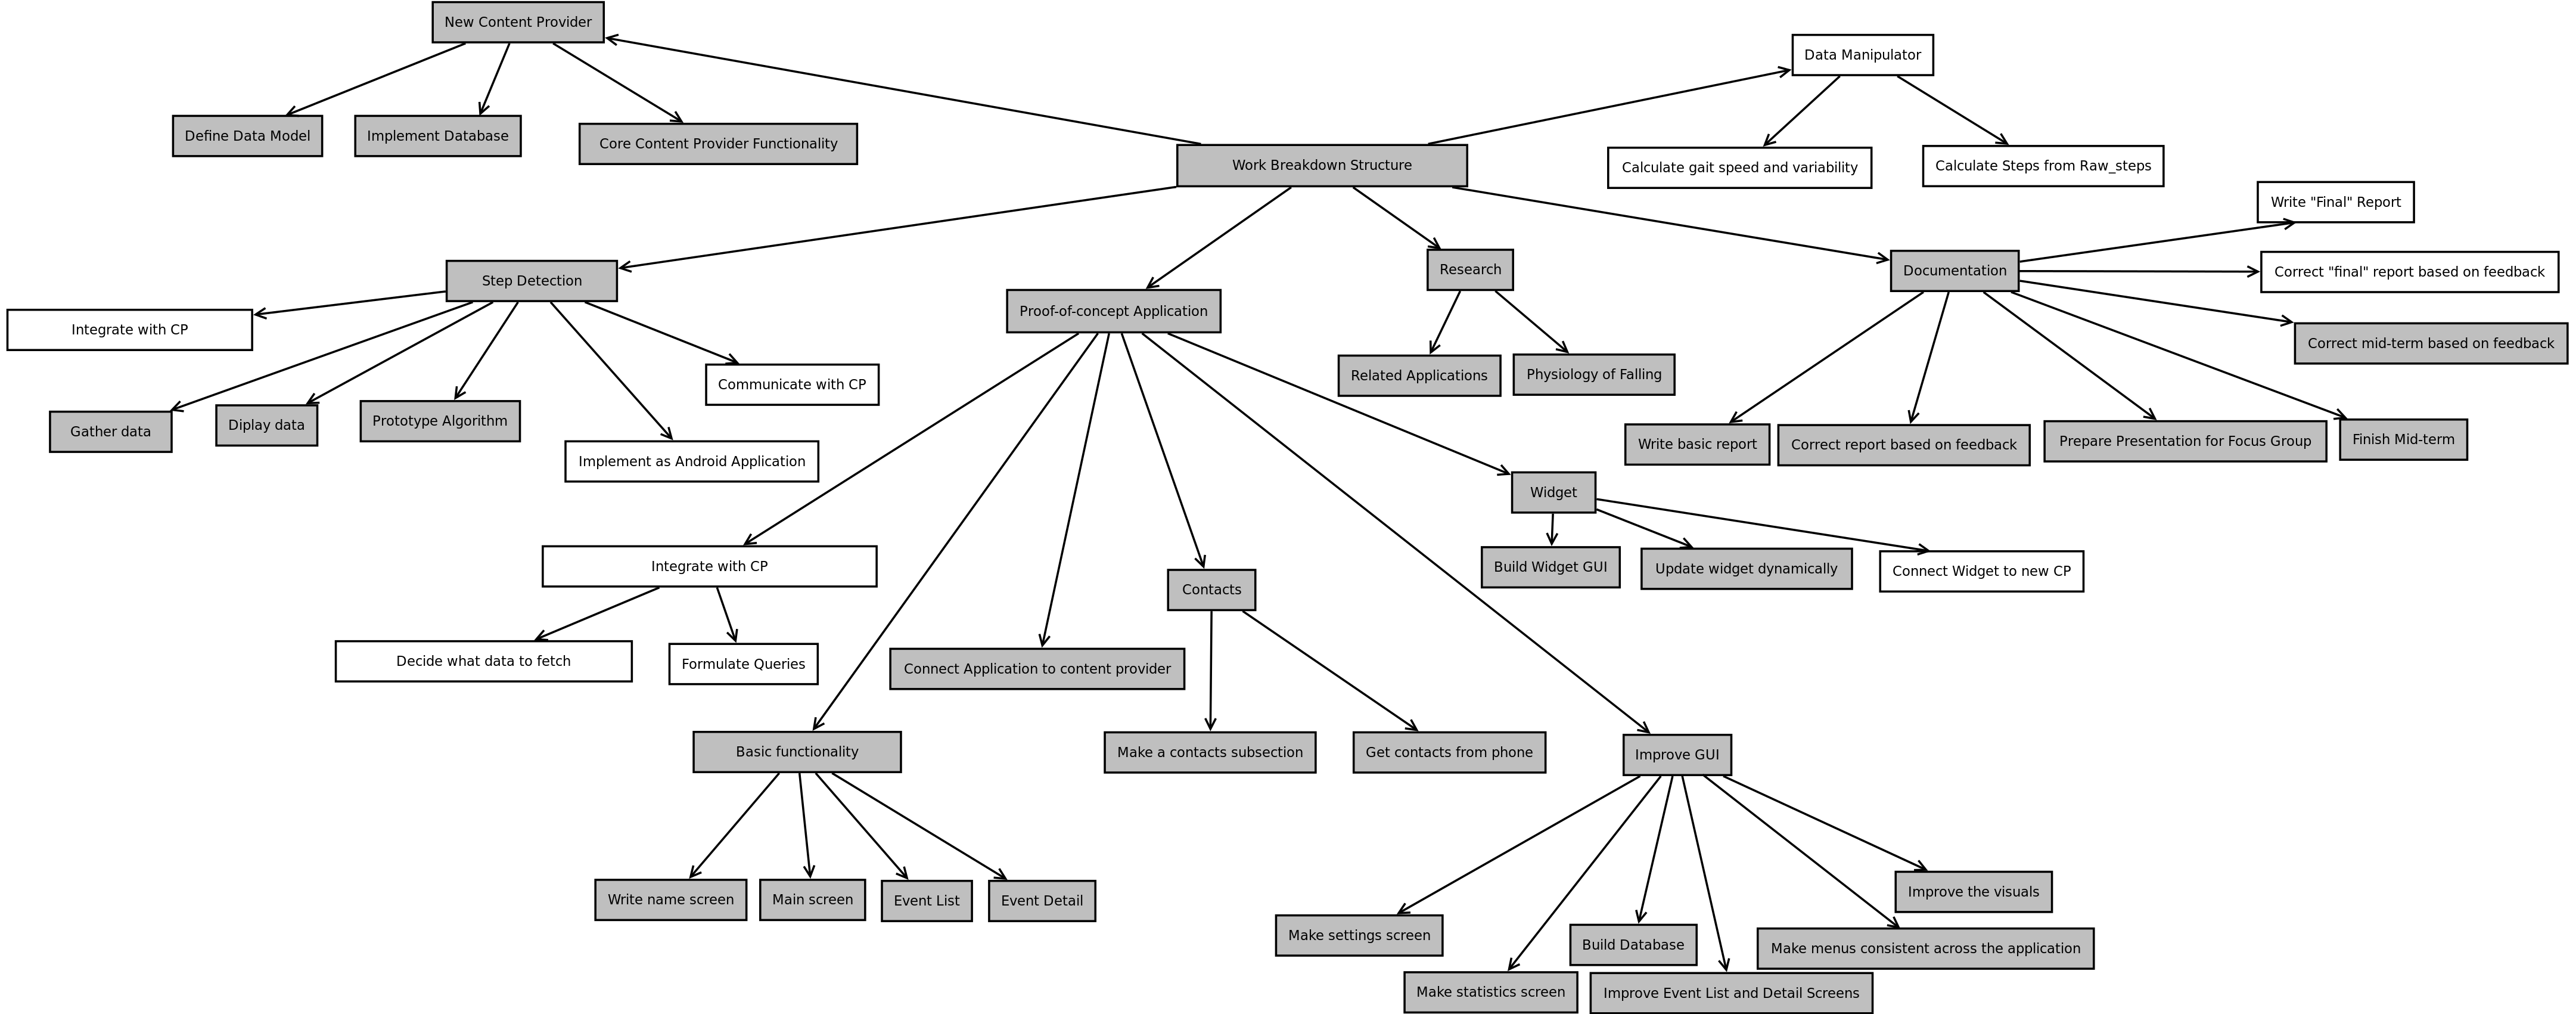
\includegraphics[width=1.45\textwidth , angle=270]{Res/WBSlast.png}
}
}

\caption{The final WBS}
\label{fig:WBS}
\end{figure}
